\chapter{Konzeption und Implementierung}
\label{sec:kzimp}
In diesem Kapitel werden die Konzeptentwicklung sowie die Technologieauswahl und die Implementierung des GuttenBase-Plugins erläutert.
\section{Konzeptentwicklung}
	
	In diesem Kapitel werden die grundlegenden Aspekte der Softwarearchitektur des GuttenBase-Plugins vorgestellt. Diese wurden basierend auf der Empfehlung im IEEE-Standard IEEE STD 1471-2000 erstellt.\\
	Die Architektur wird aus zwei Sichten (Views) betrachtet. Jede Sicht stellt dabei spezifische Informationen bereit.\\
	Es ist außerdem zu beachten, dass sich die Architektur auf die Ergebnisse der funktionalen Anforderungsanalyse sowie auf die Architektur der Zielplattform (IntelliJ-Plattform) bezieht.\\
	Im Folgenden werden die Sichten vorgestellt.

	\subsection{Konzeptionelle Sicht}
	In diesem Abschnitt wird die konzeptionelle Sicht des Systems präsentiert. Dabei wird das System noch unabhängig von den Implementierungsentscheidungen betrachtet. \\
	Die konzeptionelle Sicht wird als Komponentendiagramm in Abbildung \ref{img:component-diagram} dargestellt. 
	\begin{figure}[H]
		\centering
		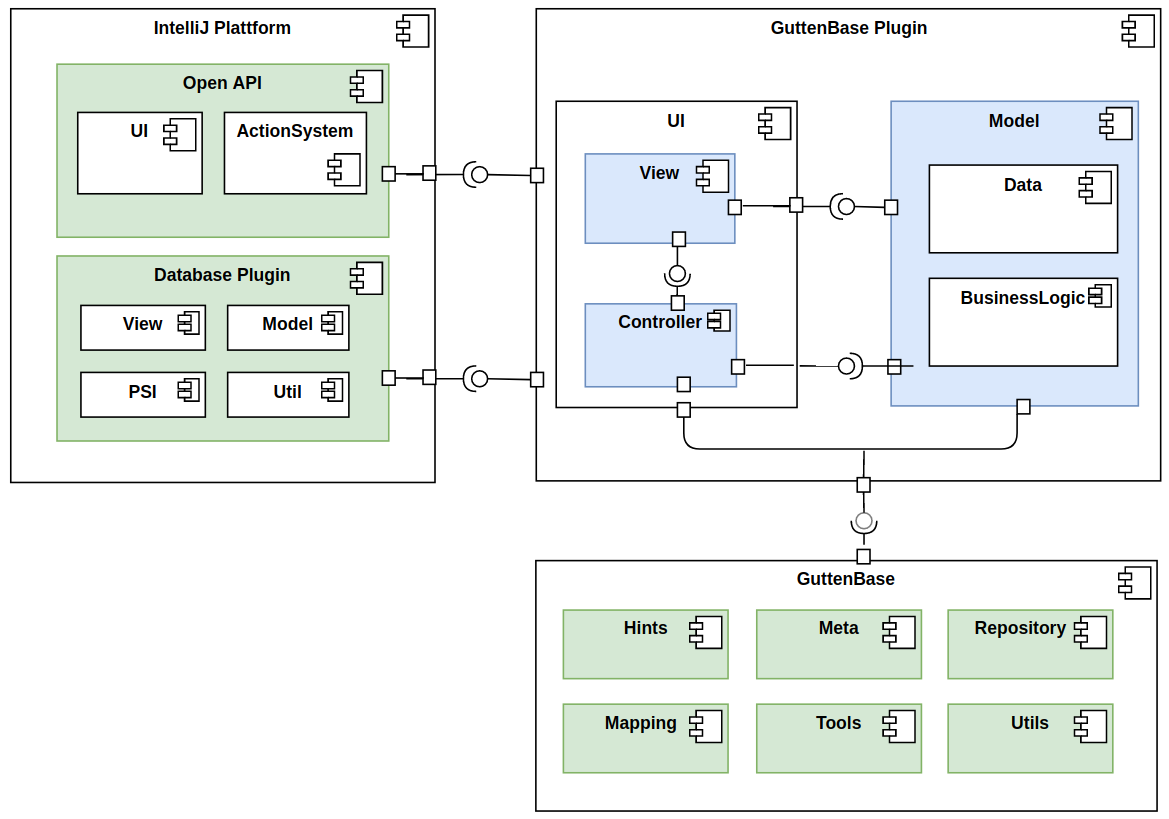
\includegraphics[width=\textwidth]{images/sichten/component-diagram}
		\caption{Komponentendiagramm für die konzeptionelle Sicht}
		\label{img:component-diagram}
	\end{figure}
	Das Komponentendiagramm besteht aus der GuttenBase-Plugin-Komponente, die das zu entwickelnde System darstellt, der IntelliJ-Plattform-Komponente und der GuttenBase-Komponente. Es werden lediglich Komponenten veranschaulicht, die vom System benötigt werden.	Diese werden im Folgenden beschrieben.
	
	\subsubsection{GuttenBase-Plugin}
	Das GuttenBase-Plugin wird nach dem MVC-Architekturstil konzipiert und besteht aus den folgenden Komponenten:
	
	\paragraph*{Model}
	Das Modell enthält Daten, die von der View-Komponente dargestellt werden. Hier befindet sich außerdem die Geschäftslogik (,Businesslogik‘), die für die Änderung der Daten zuständig ist.
	
	\paragraph*{View}
	Die \textbf{View}-Komponente ist für die Darstellung der Daten für den Benutzer verantwortlich. Hier werden alle UI-abhängigen Aspekte wie Layout, Schriftart usw. behandelt.\\
	
	\paragraph*{Controller}
	Die \textbf{Controller}-Komponente ist für die Interaktion mit dem Benutzer verantwortlich. Sie wird von der View-Komponente über Benutzerinteraktionen informiert und wertet diese aus. Anschließend können Änderungen an den Daten der Modell-Komponente sowie Anpassungen an der View-Komponente vorgenommen werden.
	
	\subsubsection{IntelliJ Plattform}
	Wie in Abbildung \ref{img:component-diagram} zu sehen ist, interagiert das GuttenBase-Plugin mit mehreren Komponenten der IntelliJ-Plattform. Es werden dabei lediglich die verwendeten Komponenten dargestellt.
	Diese sind die folgenden:
	
	\paragraph*{Open API}
	Das IntelliJ-Open-API beinhaltet zahlreiche Komponenten, die auch von der IntelliJ-IDEA-Community-Edition verwendet werden und für Plugin-Entwickler zur Verfügung stehen. Es können z. B. UI-Komponenten aus der Komponente \textbf{UI} für die Implementierung des Plugins benutzt werden. Außerdem wird die \textbf{Action-System}-Komponente benötigt, um Aktionen wie das Starten des Plugins auszulösen.
	
	\paragraph*{Database-Plugin}
	Da das GuttenBase Plugin viel mit den Datenbanken umgeht, die in IntelliJ konfiguriert wurden, ist eine Interaktion mit dem Database Plugin sehr sinnvoll. Dazu bieten sich viele Komponenten für unterschiedliche Zwecke. Die für das GuttenBase Plugin benötigten Komponenten sind die \textbf{Model} Komponente (um evt. eine Datenbank Konfiguration zu bekommen), die \textbf{PSI} Komponente (um die Elemente der Datenbank zu bekommen), die \textbf{Util} Komponente (um ein Datenbank-Schema zu bekommen) und die \textbf{View} Komponente (um aus der Übersicht des Database  Plugins Datenbank-Inhalte zu bekommen).
	
	Da das GuttenBase-Plugin mit Datenbanken interagiert, die in IntelliJ konfiguriert wurden, ist eine Interaktion mit dem Database-Plugin sinnvoll. Dazu bieten sich zahlreiche Komponenten für unterschiedliche Zwecke an. Die für das GuttenBase-Plugin benötigten Komponenten sind die \textbf{Modell}-Komponente (um eventuell eine Datenbankkonfiguration zu bekommen), die \textbf{PSI}-Komponente (um die Elemente der Datenbank zu erhalten), die \textbf{Util}-Komponente (um ein Datenbankschema zu erlangen) und die \textbf{View}-Komponente (um aus der Übersicht des Database-Plugins Datenbankinhalte zu erhalten).
	
	
	\subsubsection{GuttenBase} 
	\paragraph*{Repository}
	Unter der Repository-Komponente befindet sich das Connector-Repository, das Informationen über die Quell- und Zieldatenbank sowie die konfigurierten Migrationsoperationen enthält. Das Connector-Repository wird während der gesamten Migration vom GuttenBase-Plugin verwendet.
	\paragraph*{Meta}
	Hier sind Klassen enthalten, die die Datenbankelemente (Schemata, Tabellen und Spalten) darstellen.
	\paragraph*{Hints}
	Die Hints Komponente enthält die Standardimplementierung der Migrationsoperationen (z. B. Tabellenumbenennung). Diese können während der Migration überschrieben werden.
	\paragraph*{Mapping}
	Hier befinden sich alle Mapper Klassen. Diese können beim Konfigurieren der Migrationsoperationen benutzt werden.
	\paragraph*{Tools}
 	Die Tools-Komponente übernimmt das Ausführen bestimmter Aufgaben, etwa das Kopieren der Tabellen während der Migration.
 	\paragraph*{Utils}
	Unter Utils liegen Klassen, die für das Logging des Migrationsprozesses benötigt werden. Beispielsweise kann die Logging-Script-Executor-Progress-Indicator-Klasse genutzt werden, um relevante Informationen über den Migrationsprozess (z. B. die verstrichene Zeit oder die aktuelle SQL-Anfrage) zu erhalten.
	Diese können für das Darstellen des Migrationsfortschrittes verwendet werden.
	
	
	
	\subsection{Modulsicht}
	Die Modulsicht zeigt die Struktur des GuttenBase-Plugins in Form von Modulen und deren Beziehungen zueinander. Dabei werden die Komponenten und Konnektoren der konzeptionellen Sicht auf Module, Schichten und Subsysteme abgebildet. Diese werden in Paket- und Klassendiagrammen verfeinert. Zur Wahrung der Übersichtlichkeit wird die Modulsicht nach den verschiedenen Übersichten unterteilt. Es gibt insgesamt vier Übersichten, die das gesamte System abdecken. Pro Übersicht werden lediglich Klassen bzw. Methoden beschrieben, die die entsprechenden Anwendungsfälle realisieren.
	
	\subsubsection{Modulsicht der Übersicht über die Migrationsoperationen}

	Die Modulsicht in Abbildung \ref{img:modulsicht-gbactions} beinhaltet alle beteiligten Klassen, die beim Erstellen und Verwalten der Migrationsoperationen eingesetzt werden. Diese werden entsprechend der konzeptionellen Sicht aufgeteilt, nämlich in die View-, Modell- und Controller-Pakete.
	
	
	%-View Klassen sind für die UI - Swing KOmponenten.
	%- Controlle hat folgende Aufgaben: 
	%- UI Komponenten erstellen, 
	%- Aktionen erstellen: die GBActionView informiert controller über Benutzer Eingabe -> jenachdem welchen ActionTyp selektiert wurde, wird die entsprechende DumbAwareAction ausgeführt, damit die entsprechende Dialoge für das Erstellen der Action angezeigt wird (renameView + changeType))
	%- editieren und speichern: nach dem Klick auf Save wird die Save Methode des Controller aufgerufen, sodass alle hinzugefügten Migrationsoperationen mithilfe der GsonHelper konvertiert und gespeichert werden.
	%- actionen darstellen, 
	%- Übersicht schließen: Nach dem Klick auf cancel wird die Übersicht geschlossen.
	\begin{figure}[H]
		\centering
		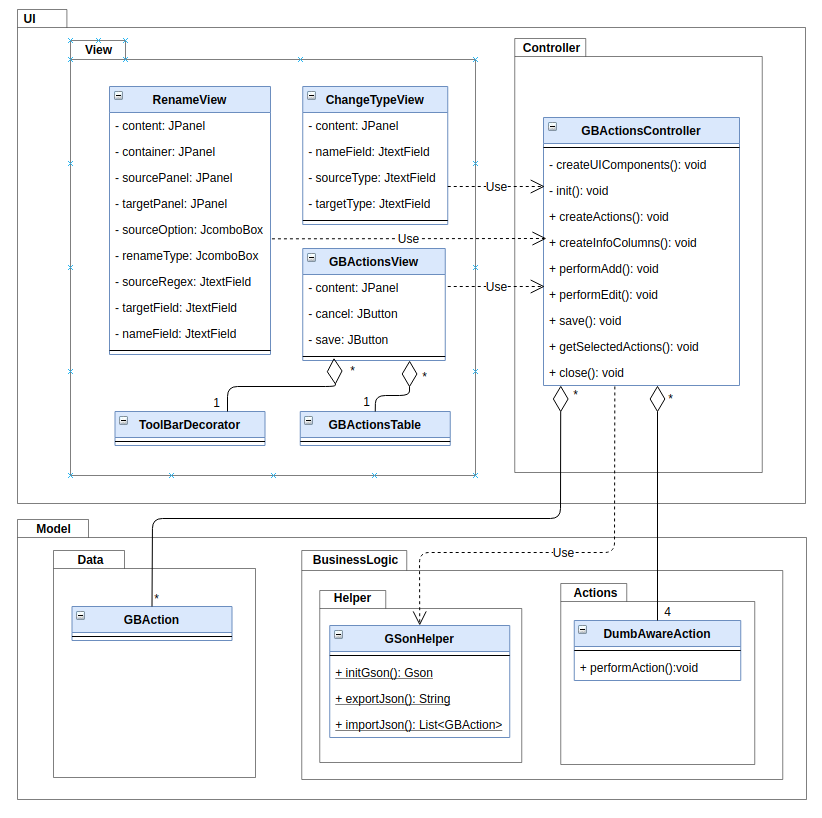
\includegraphics[width=\textwidth]{images/sichten/modulsicht-gbactions}
		\caption{Modulsicht der Übersicht über die  Migrationsoperationen}
		\label{img:modulsicht-gbactions}
	\end{figure}
	Im View-Paket werden alle Klassen dargestellt, die für die Abbildung der Migrationsoperationen zuständig sind. Sie basieren auf unterschiedlichen Swing-Komponenten. Die Klasse GB-Actions-View repräsentiert dabei die Hauptübersicht der Migrationsoperationen und beinhaltet die GB-Actions-Table-Klasse, die die Auflistung der Migrationsoperationen übernimmt. Außerdem wird die Toolbar-Decorator-Klasse für die Darstellung der möglichen Aktionen benötigt.\\
	Das Controller-Paket enthält die GB-Actions-Controller-Klasse. Diese hat die folgenden Aufgaben:
	\begin{itemize}
		\item UI-Komponenten vor dem Anzeigen vorbereiten, indem Daten aus dem Paketmodell erzeugt bzw. geladen werden.
		\item Migrationsoperationen erstellen: Dies geschieht, wenn der Benutzer eine bestimmte Migrationsoperation hinzufügen möchte und diese in der GB-Actions-View-Übersicht selektiert. Zunächst wird die entsprechende Dumb-Aware-Action-Klasse aufgerufen, um die entsprechende Aktion durchzuführen. Die Dumb-Aware-Action-Klasse ist im Paket BusinessLogic zu finden und kann für das Erstellen von Migrationsoperationen verwendet werden. Diese werden durch die Rename-View- und die Change-Type-View-Klassen realisiert. Analog dazu erfolgt das Editieren der Migrationsoperationen.
		\item Die Migrationsoperationen werden gespeichert, indem die hinzugefügten Migrationsoperationen in JSON konvertiert und dann exportiert werden. Dafür ist die Gson-Helper-Klasse des Business-Logic-Pakets zuständig.
	\end{itemize}
	
	
	
	\subsubsection{Modulsicht der allgemeinen Übersicht}
	Diese Modulsicht zeigt die beteiligten Klassen, die beim Verbinden der zu migrierenden Datenbanken genutzt werden, und ist in Abblidung \ref{img:modulsicht-general} dargestellt. 
	\begin{figure}[H]
		\centering
		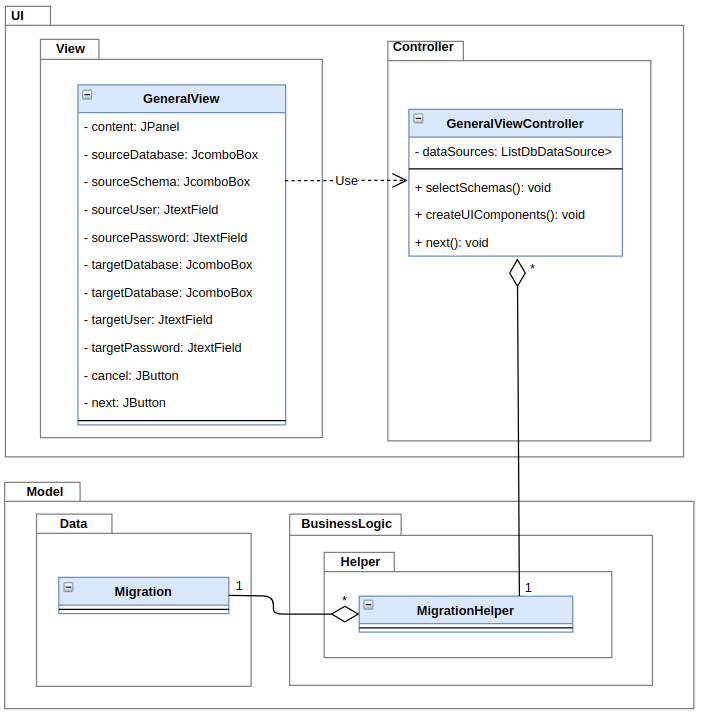
\includegraphics[width=0.7\textwidth]{images/sichten/modulsicht-general}
		\caption{Modulsicht der allgemeinen Übersicht}
		\label{img:modulsicht-general}
	\end{figure}
	Die General-View-Klasse ist für die Interaktion mit dem Benutzer verantwortlich und enthält alle Eingabefelder und Texte. Die General-View-Controller-Klasse ist für das Laden der Datenbankelemente zuständig. Klickt der Benutzer auf den ‚Next‘-Button, werden alle Eingaben über die Migration-Helper-Klasse des Pakets BusinessLogic übergeben. Diese Informationen werden dann in der Migrationsklasse des Modellpakets gespeichert.
	
	\subsubsection{Modulsicht der Konfigurationsübersicht}
	Die Modulsicht in  Abbildung \ref{img:modulsicht-overview} zeigt die für die Konfigurationsübersicht relevanten Klassen.
	\begin{figure}[H]
		\centering
		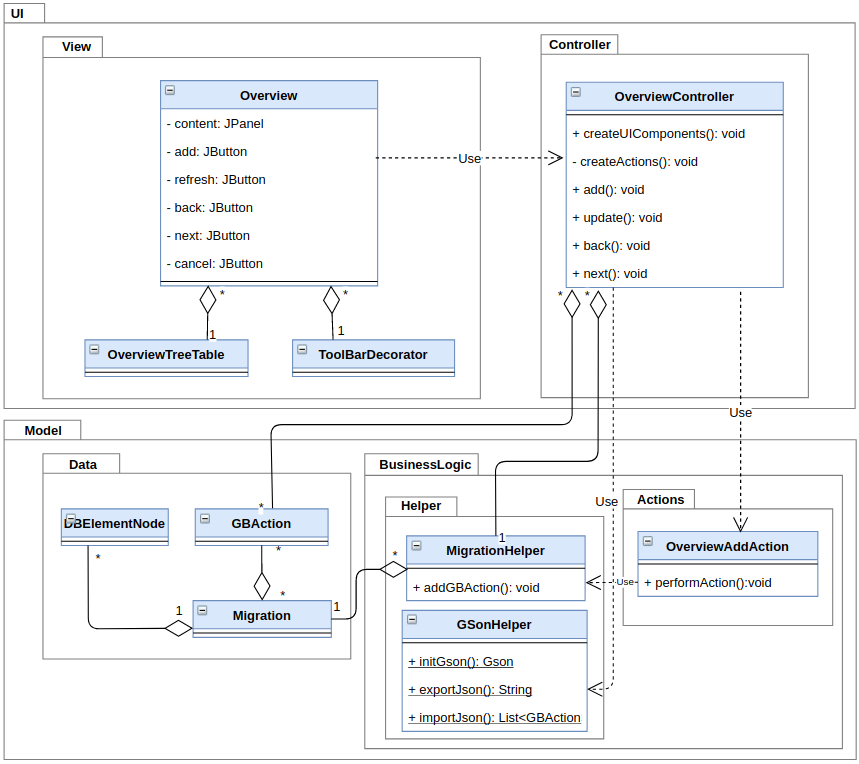
\includegraphics[width=\textwidth]{images/sichten/modulsicht-overview}
		\caption{Modulsicht der Konfigurationsübersicht}
		\label{img:modulsicht-overview}
	\end{figure}
	Die Konfigurationsübersicht (Overview) enthält die Overview-Tree-Table-Klasse, die alle	Quelldatenbankelemente auflistet, und die Toolbar-Decorator-Klasse, die die gespeicherten Migrationsoperationen anzeigt. Außerdem stehen einige Buttons für die Benutzerinteraktion zur Verfügung. \\
	Wie bei den bereits erläuterten Modulsichten stellt die Overview-Controller-Klasse Methoden für die folgenden Zwecke bereit:
	\begin{itemize}
		\item Das Laden der Datenbankelemente: Hierbei werden die gespeicherten Migrationsoperationen mithilfe der Gson-Helper-Klasse importiert und die Datenbankelemente (DBElementNode) aus der Quelldatenbank erstellt.
		\item Das Anzeigen der Migrationsoperationen: Die Migrationsoperationen werden nach ihrer Kompatibilität mit den selektierten Datenbankelementen behandelt. Ist eine Migrationsoperation für ein Datenbankelement geeignet, wird diese klickbar angezeigt. Ansonsten wird ein ausgegrauter Button dargestellt.
		\item Hinzufügen von Migrationsoperationen: Wenn der Benutzer ein Datenbankelement selektiert und dann eine entsprechende Migrationsoperation hinzufügt, wird die Overview-Add-Action-Aktion vom Business-Logic-Paket ausgelöst. Dabei wird die entsprechende Migrationsoperation von der Migration-Helper-Klasse der Migration hinzugefügt.
	\end{itemize}
	
	
	
	\subsubsection{Modulsicht der Ergebnisübersicht}
	Die Modulsicht in Abbildung \ref{img:modulsicht-resul} stellt die für die Ergebnisübersicht (ResultView) zuständigen Klassen dar. Außerdem wird die Fortschrittübersicht (ProgressView) miteingebunden, da diese vom selben Controller verwaltet wird.
	\begin{figure}[H]
		\centering
		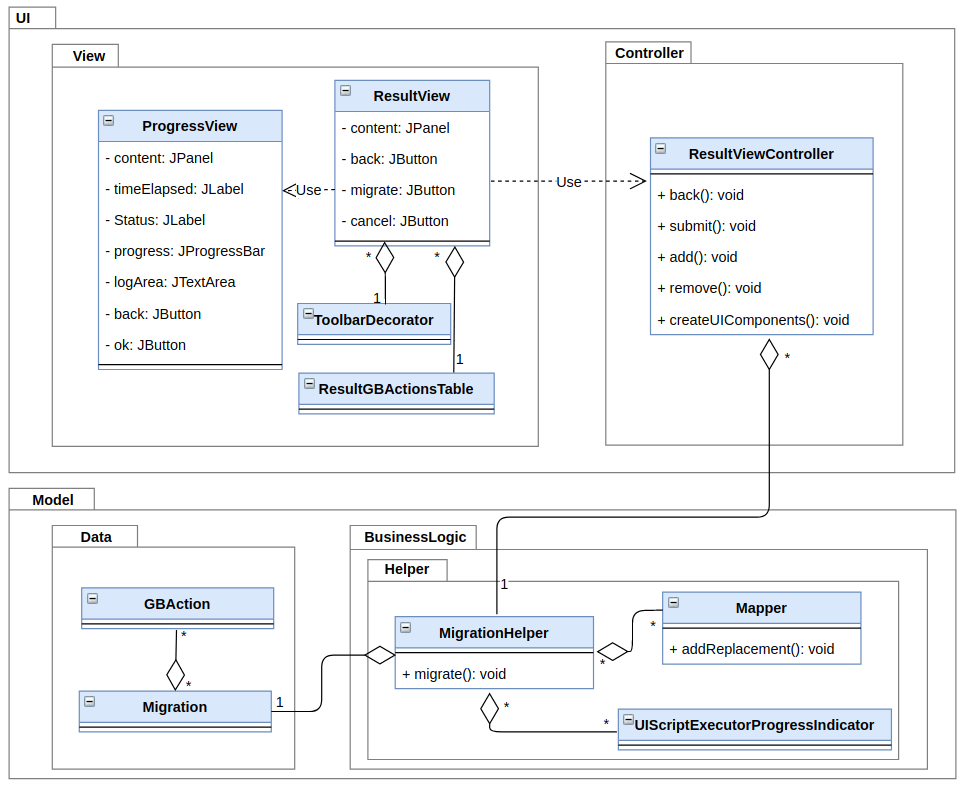
\includegraphics[width=\textwidth]{images/sichten/modulsicht-result}
		\caption{Modulsicht der Ergebnisübersicht}
		\label{img:modulsicht-resul}
	\end{figure}
	
	Ähnlich wie bei den anderen Übersichten enthält die Result-View-Klasse eine Tabelle (ResultGBActionsTable), die alle hinzugefügten Migrationsoperationen enthält, und einen ToolbarDecorator, wo die Aktionen zum Löschen und Hinzufügen angezeigt werden. \\
	Auf der anderen Seite stellt die Result-View-Controller-Klasse Methoden für das Löschen und das Hinzufügen von Migrationsoperationen sowie für das Starten des Migrationsprozesses bereit. Diese werden im Folgenden erklärt:
	
	\begin{itemize}
		\item Hinzufügen: Wenn der Benutzer weitere Migrationsoperationen zur Migration hinzufügen möchte, wird die aktuelle Übersicht zur Übersicht der Migrationsoperationen (Overview) umgeleitet.
		
		\item Löschen: Wie das Hinzufügen erfolgt das Löschen von Migrationsoperationen (die bereits zur Migration hinzugefügt wurden) durch die Entfernung der ausgewählten Migrationsoperation (GBAction) aus der Migrationsklasse.
		
		\item Migration starten: Nach einem Klick auf den ,Migrate‘-Button wird der Migrationsprozess gestartet. Dieser erfolgt mittels der Migration-Helper-Klasse. Dabei wird das Connector-Repository der GuttenBase-Bibliothek entsprechend den Migrationsoperationen konfiguriert (siehe \ref{section:grundlagen:gb}) und anschließend das Kopieren vom Default-Table-Copy-Tool gestartet.\\
		Parallel dazu wird die Fortschrittübersicht (ProgressView) angezeigt, um Informationen über den laufenden Prozess zu erhalten. Dies wird durch die UI-Script-Executor-Progress-Indicator-Klasse ermöglicht.
		
		%	- add connectors, cfg abgeschlossen -> Copy 
		%	- parallel dazu: Fortschritt übersicht anzeigen: Logginging: Logging Hin.
	\end{itemize}


\section{Technologieauswahl}
	IIm Folgenden wird die Umsetzungsform des GuttenBase-Plugins begründet. Außerdem werden die Nutzung der GuttenBase-Bibliothek und die IntelliJ-Plugin-Entwicklung beschrieben.
\subsection{Umsetzungsform}

Um eine optimale Nutzung des GuttenBase-Plugins zu gewährleisten, muss auf die Umsetzungsform geachtet werden.\\
Das zu entwickelnde Tool kann z. B. als eine Desktopapplikation, Webapplikation oder als Plugin einer anderen Anwendung realisiert werden.\\
In Tabelle \ref{table:tool-options} werden die Eigenschaften einer jeden Alternative erläutert.\\
Alle drei Optionen weisen Vor- und Nachteile auf, allerdings sind die raschere Erreichung zahlreicher Nutzer sowie die einfache Installation bei der IDE-Plugin-Entwicklung entscheidend.
\begin{table}
	\centering
	\caption{Umsetzungsmöglichkeiten}
	\begin{tabular}{ |p{3cm}|p{6cm}|p{6cm}| }
		\hline
		\textbf{Alternative} & \textbf{Vorteile} &  \textbf{Nachteile}  \\
		Desktop-App & 
		\begin{itemize}
			\item Offline immer verfügbar
			\item Vollständige Kontrolle über die Anwendung und die enthaltenen Daten.
			\item Höhere Leistung, da kein Browser als Zwischenschicht existiert.
		\end{itemize}& 
		\begin{itemize}
			\item Platformabhängig
			\item Hohe Entwicklungskosten
			\item Installation ist notwendig
		\end{itemize} \\
		\hline
		Web-App &
		
		\begin{itemize}
			\item Eine Installation oder manuelle Updates sind nicht notwendig. 
			\item Geringere Entwicklungs- und Wartungskosen, da die Anwendung unabhängig von lokalen Endgeräten ist.
		\end{itemize} &
		
		\begin{itemize}
			\item Offline meist nicht verfügbar.
			\item Niedrigere Leistung.
		\end{itemize} \\
		\hline
		IDE-Plugin-Entwicklung &
		
		\begin{itemize}
			\item Für IntelliJ Benutzer  einfach und intuitiv zu benutzen.
			\item Manche Komponenten bzw. Funktionalitäten der zu erweiternden IDE können wiederverwendet werden, was die Entwicklungsdauer verkürzt.
			\item Intuitive Nutzung sowie eine einheitliche Benutzeroberfläche wie bei der benutzten IDE.
		\end{itemize} &
		
		\begin{itemize}
			\item Die Flexibilität beim Entwickeln ist durch die limitierte Erweiterbarkeit der IDE eingeschränkt.
		\end{itemize} \\
		\hline
		
	\end{tabular}
	\label{table:tool-options}
\end{table}

Zunächst muss eine Entscheidung für eine konkrete IDE getroffen werden. Um eine IDE auszuwählen, muss auf die Anzahl der Nutzer, die Verfügbarkeit der Dokumentation für die Plugin-Entwicklung sowie die Unterstützung von Datenbanken geachtet werden.\\
Eine der bekanntesten Methoden, um die Beliebtheit einer Programmiersprache bzw. einer IDE herauszufinden, ist der PYPL-Index. Er basiert auf Rohdaten aus Google Trends. PYPL enthält den TOP-IDE-Index, mit dem analysiert wird, wie häufig IDEs bei Google gesucht werden. Die Suchanfragen spiegeln zwar nicht unbedingt die Beliebtheit der IDEs wider. Dennoch hilft ein solcher Index bei der Wahl einer Entwicklungsumgebung. Bei dieser Analyse sind die drei bekanntesten und für den vorliegenden Fall relevanten Entwicklungsumgebungen Visual Studio (erster Platz), Eclipse (zweiter Platz) und IntelliJ (sechster Platz). Außerdem ist der Index von IntelliJ IDE am meisten gestiegen (siehe Abbildung \ref{img:ide-index}).\\
Bei einer Untersuchung (Jaxenter) zu der Frage, mit welcher Entwicklungsumgebung am ehesten in Java programmiert wird, war IntelliJ auf dem ersten Platz mit 1660 von 2934 Stimmen.

\begin{figure}[H]
	\centering
	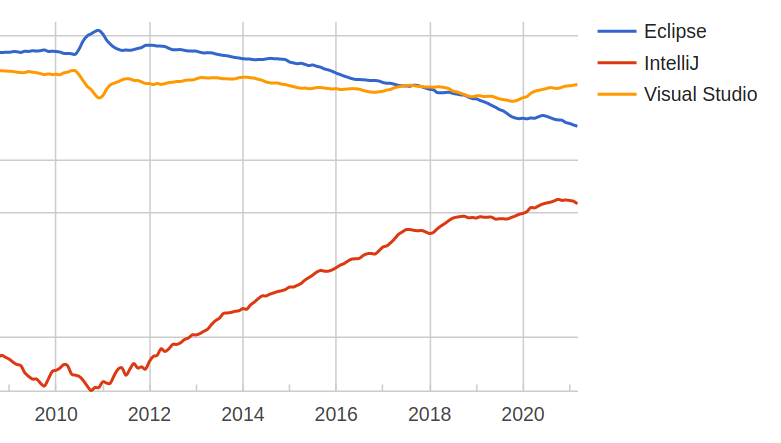
\includegraphics[width=0.8\textwidth]{images/ide-index}
	\caption{Top-IDE-Index}
	\label{img:ide-index}
\end{figure}
Aus den oben erläuterten Daten und aufgrund der hinreichenden Dokumentation für die Plugin-Entwicklung wird das GuttenBase-Plugin als ein Intellij-Plugin umgesetzt.

\subsection{IntelliJ Platform}
	Für eine erfolgreiche IntelliJ-Plugin-Entwicklung muss auf mehrere Aspekte geachtet werden, etwa auf die Projektstruktur und die häufig verwendeten Komponenten. \\
	Die Plugin-Entwicklung erfolgt in der IntelliJ-IDE selbst. Daher kann das Plugin entweder in Java, Kotlin, Groovy oder Scala geschrieben werden.\\
	Der von Jetbrains empfohlene Weg für das Erstellen eines neuen Plugins ist das Gradle-Projekt. Dabei muss die Option ,IntelliJ Platform Plugin‘ ausgewählt werden, damit die Plugin-Abhängigkeiten sowie die Basis-IDE automatisch konfiguriert werden. Zusätzlich muss die Datei plugin.xml entsprechend dem zu entwickelnden Plugin angepasst werden. Diese Datei enthält zentrale Informationen, die in den folgenden Tags (Auszeichnungen) erklärt werden:
	\begin{itemize}
		\item \textbf{<name>} \\
		Der Name des Plugins; er soll kurz und beschreibend sein.
		\item \textbf{<id>} \\    • 
		Eine eindeutige Bezeichnung des Plugins; diese kann nicht während der Entwicklung geändert werden.
		\item \textbf{<description>} \\
		Eine Kurze Beschreibung des Plugins.
		\item \textbf{<change-notes>} \\
		Eine Beschreibung der Änderungen in der aktuellen Version des Plugins.
		\item \textbf{<version>} \\    • 
		Die aktuelle Plugin-Version.
		\item \textbf{<vendor>} \\    • 
		Der Anbieter des Plugins; hier kann zusätzlich eine E-Mail-Adresse angegeben werden.
		\item \textbf{<depends>} \\    • 
		Abhängigkeiten von Plugins oder Modulen.
		\item \textbf{<idea-version>} \\    • 
		Die minimale und maximale Version der IDE, mit der das Plugin kompatibel ist.
		\item \textbf{<actions>} \\    • 
		Mit diesem Tag wird definiert, wie die Funktionalität des Plugins aufgerufen wird. Dies wird im folgenden Abschnitt behandelt.
		\item \textbf{<extensionPoints>} \\    • 
		Die vom Plugin definierten Erweiterungspunkte. Diese können es anderen Plugin-Entwicklern erlauben, auf bestimmte Daten zuzugreifen.
		\item \textbf{<extensions>} \\    • 
		Erweiterungspunkte, die von der IntelliJ-Platform bzw. von anderen Plugins definiert sind und von dem zu entwickelnden Plugin verwendet werden.
	\end{itemize}
	\subsubsection*{Action-System}
	Die am häufigsten verwendete Methode, um die Plugin-Funktionalität aufzurufen, ist die Nutzung der sogenannten ,Actions‘ des Action-Systems der IntelliJ-Platform.\\
	Eine Aktion kann über einen Menüpunkt (menu item) oder einen Eintrag in der Symbolleiste ausgelöst werden. Dazu muss ein Eintrag in den Actions-Tag der plugin.xml-Datei erfolgen. Dabei muss jede Aktion mindestens eine ID, eine Klasse und einen beschreibenden Text aufweisen. In der Regel werden Menüpunkte nach deren Funktionalität gruppiert. Um die Implementierte Aktion einer bestimmten Gruppe hinzufügen zu können, muss der Tag ,<add-to-group>‘ verwendet werden.\\
	Die Action-Klasse muss von der An-Action-Klasse abgeleitet werden und die actionPerformed()-Methode überschreiben. Diese wird nach dem Klick auf den entsprechenden Menüpunkt bzw. auf die Symbolleiste aufgerufen.
	%\subsubsection{Swing}
	%TODO TEST
	%\subsubsection{IntelliJ Plugin Entwicklung}
	
	
	
	
	
	
\subsection{GuttenBase}
	\label{sec:imp:gb}
%	Die Nutzung der GuttenBase Bibliothek wird in folgenden Schritten erklärt.
	%\subsection{Schritt 1: Abhängigkeiten}
	%Um GuttenBase verwenden zu können, soll werden folgende Informationen benötigt:
	%\begin{itemize}
	%	\item groupId: de.akquinet.jbosscc.guttenbase
	%	\item artifactId: GuttenBase
	%	\item version: 2.0.0
	%\end{itemize}
	%Außerdem 
%	\paragraph*{Schritt 1: Datenbankverbindung erstellen}
	Für die Nutzung der GuttenBase-Bibliothek sollen zunächst Abhängigkeiten zum laufenden Projekt (z. B. Gradle) hinzugefügt werden. Die für GuttenBase benötigten Informationen sind die folgenden:
	\begin{itemize}
		\item groupId: de.akquinet.jbosscc.guttenbase
		\item artifactId: GuttenBase
		\item version: 2.0.0
	\end{itemize}
	Es ist außerdem zu beachten, dass auch die Abhängigkeiten für die Treiber-Klassen dem Quell- und Ziel-DBMS hinzugefügt werden müssen.
	
	Zunächst sollten die Connection-Info-Klassen erstellt werden. Diese beschreiben die Quell- und Zieldatenbanken und enthalten die für eine JDBC-Verbindung (Java-Database-Connectivity) erforderlichen Attribute.\\
	\begin{figure}[H]
		\centering
		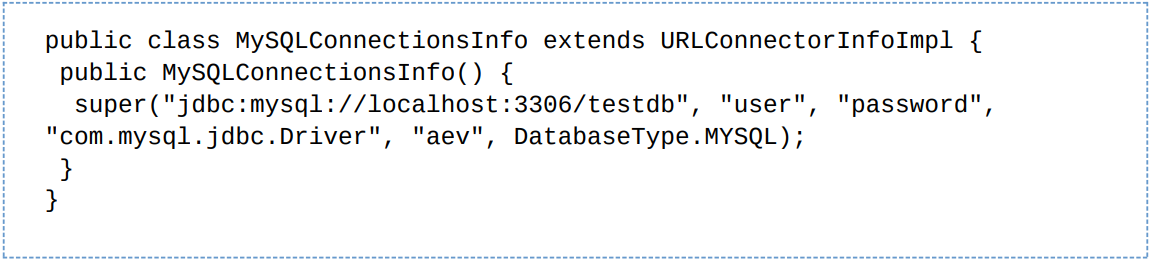
\includegraphics[width=0.8\textwidth]{images/gb/conInfo}
		\caption{ConnectionInfo konfigurieren}
		\label{img:gb/conInfo}
	\end{figure}
	
	Im Nachhinein wird das Connector-Repository konfiguriert. Dieses enthält alle Konnektoren, die an der Datenbankmigration beteiligt sind.
	\begin{figure}[H]
		\centering
		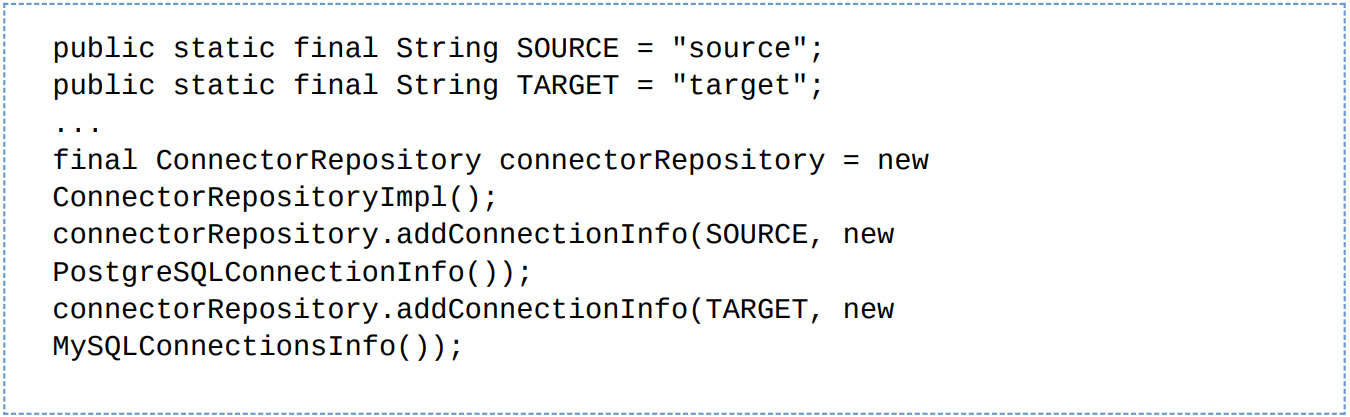
\includegraphics[width=0.8\textwidth]{images/gb/repo}
		\caption{Connector Repository konfigurieren}
		\label{img:gb/repo}
	\end{figure}
	
%	\paragraph*{Schritt 2: Hinweise hinzufügen}
	Meist werden Konfigurationshinweise (hints) benötigt, um die Migration zu individualisieren. In der Dokumentation von GuttenBase\footnote{Getting Started with GuttenBase (2018, 04.01) \\ \url{https://github.com/akquinet/GuttenBase/blob/master/Getting\%20Started\%20with\%20GuttenBase.pdf}} befindet sich eine Liste aller unterstützen Konfigurationshinweise. \\
	Als Beispiel wird der Konfigurationshinweis ColumnMapperHint in der Abbildung dargestellt.
	\begin{figure}[H]
		\centering
		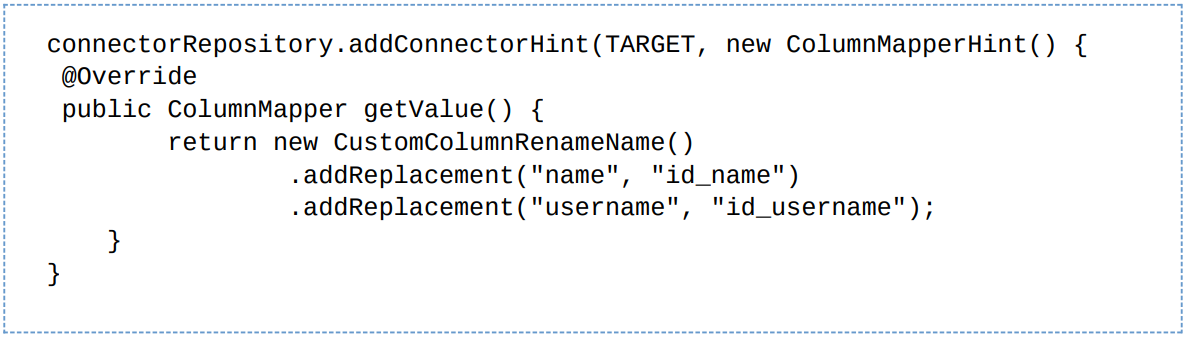
\includegraphics[width=0.8\textwidth]{images/gb/rename}
		\caption{ColumnMapperHint hinzufügen}
		\label{img:gb/rename}
	\end{figure}
	
	
%	\paragraph*{Schritt 3: Datenbank Migration durchführen}
	Anschließend kann die Migration mit den eventuell hinzugefügten Hinweisen durchgeführt werden. Dies findet wie folgt statt:
	\begin{itemize}
		\item Das Datenbankschema wird von der Quelldatenbank in die Zieldatenbank kopiert. Dabei werden möglichst viele Unterschiede in der Datentypdarstellung standardmäßig berücksichtigt.
		\item Die Kompatibilität der Schemata wird geprüft. Dabei wird nach gleichen Tabellen bzw. Spalten gesucht.
		\item Falls keine Fehler beim Prüfen auftreten, werden die Daten kopiert.
	\end{itemize}
	\begin{figure}[H]
		\centering
		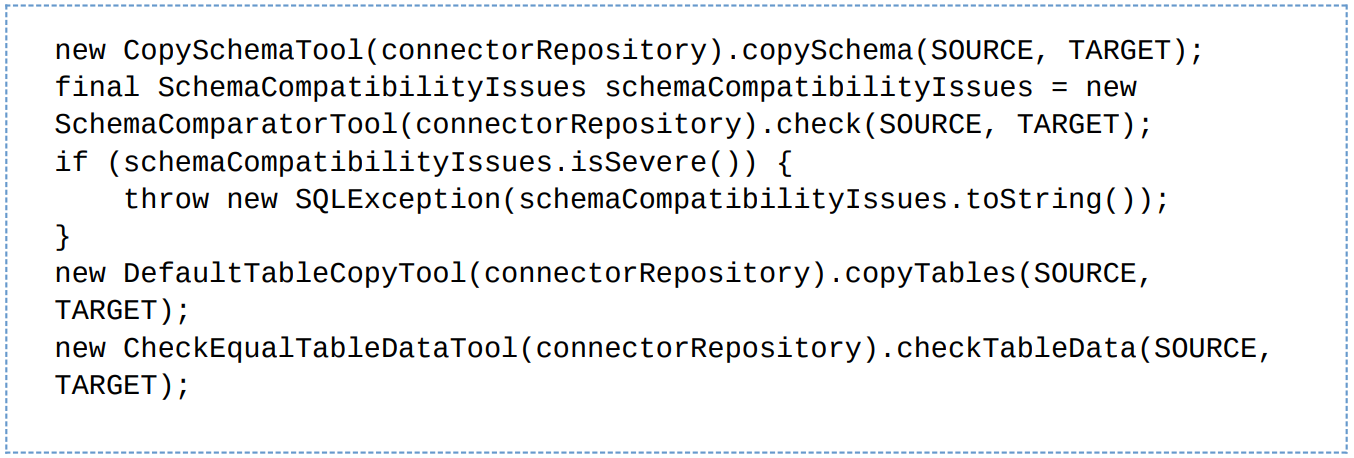
\includegraphics[width=0.8\textwidth]{images/gb/copy}
		\caption{Datenbankmigration durchführen}
		\label{img:gb/copy}
	\end{figure}
	
	
	
\section{Plugin Implementierung}
\label{sec:imp}

Dieser Abschnitt hat die Implementierung des GuttenBase-Plugins zum Thema. Die daraus resultierende Anwendungsoberfläche wird anhand der folgenden Anwendungsfunktionalitäten veranschaulicht:
\begin{itemize}
	\item Liste der vorhandenen Migrationsoperationen,
	\item Hinzufügen einer neuen Migrationsoperation,
	\item Verbindungerstellung,
	\item Konfiguration,
	\item Migrationsdurchführung.
\end{itemize}
\subsection{Funktion: Liste der vorhandenen Migrationsoperationen}

	Um die Funktionalität des GuttenBase-Plugins einfach und intuitiv für IntelliJ-Nutzer zur Verfügung zu stellen, wurden Menüpunkte zum Database-Plugin hinzugefügt. Diese wurden gemäß dem Grundsatz der Unterscheidbarkeit platziert. Somit kann die Übersicht der Migrationsoperationen nach einem Klick auf ,Show Migration Actions‘ geöffnet werden. Dies ist in Abbildung \ref{img:creategbaction} dargestellt. Diese enthält standardmäßig lediglich zwei Migrationsoperationen (Tabellen bzw. Spalten ausschließen).\\
	\begin{figure}[h]
		\centering
		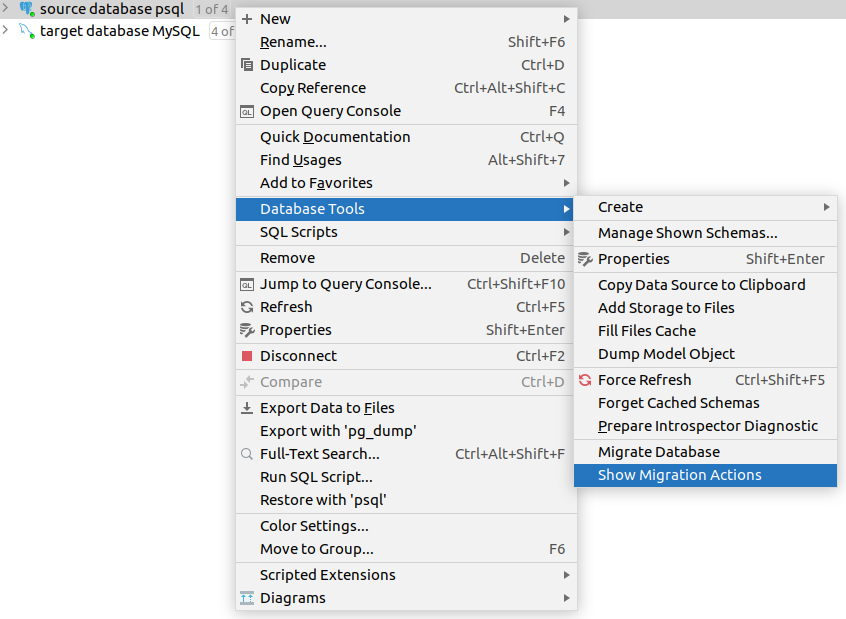
\includegraphics[width=0.7\textwidth]{images/ui/dbactions}
		\caption{Übersicht der Migrationsoperationen öffnen}
		\label{img:dbactions}
	\end{figure}
	%\begin{figure}[h]
	%	\centering
	%	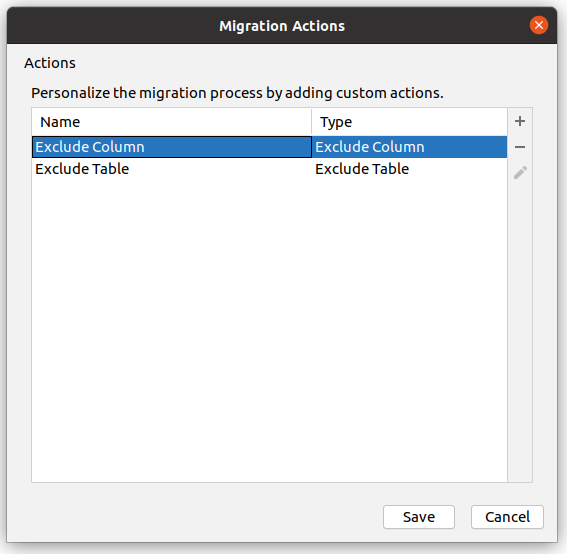
\includegraphics[width=0.5\textwidth]{images/ui/gbactions}
	%	\caption{Übersicht der Migrationsoperationen}
	%	\label{img:gbactions}
	%\end{figure}
	\begin{figure}[H]
		\centering
		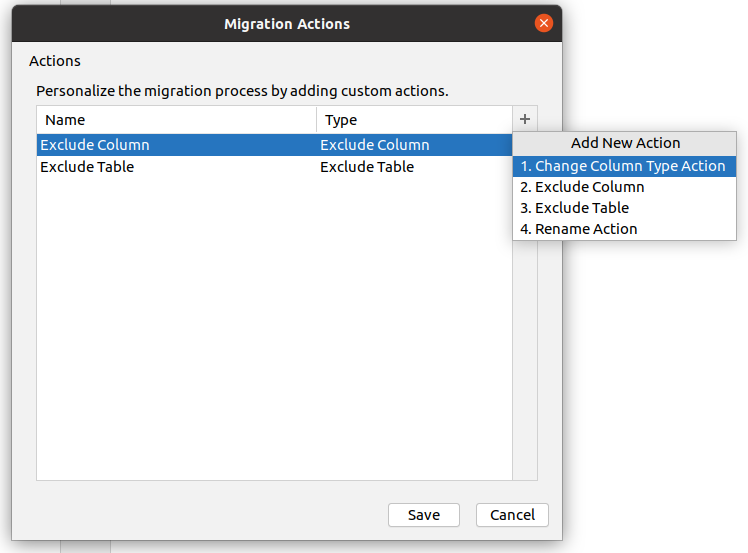
\includegraphics[width=0.7\textwidth]{images/ui/creategbaction}
		\caption{Übersicht der Migrationsoperationen}
		\label{img:creategbaction}
	\end{figure}

\subsection{Funktion: Hinzufügen einer neuen Migrationsoperation}
	
	Bei der Übersicht in der Abbildung \ref{img:creategbaction} kann der Benutzer verschiedene Migrationsoperationen erstellen, wenn diese nicht bereits existieren. In diesem Szenario wird nur das Hinzufügen von der Migrationsoperation Umbenennen (Rename Action) dargestellt.\\
	Nach dem Klick auf das entsprechende Button wird ein Dialog angezeigt, um die erforderliche Informationen einzugeben. Dabei wird der Name der Migrationsoperation festgelegt. Außerdem der Quell-Name durch einen regulären Ausdruck definiert. Anschließend  wird die der Zeil-Name festgelegt. \\
	Die in der Abbildung \ref{img:createRename} angezeigte Migrationsoperation gilt für alle Datenbankelemente, deren Name die Zeichenkette \glqq table\grqq enthält. Wenn diese an einem entsprechenden Datenbankelement angewendet wird, wird das Suffix \glqq \_Test\grqq \, hinten hinzugefügt.
	
	
	Mittels der Übersicht in Abbildung  \ref{img:creategbaction} kann der Benutzer verschiedene Migrationsoperationen erstellen, sofern solche nicht bereits existieren. In diesem Szenario wird lediglich das Hinzufügen der Migrationsoperation ,Umbenennen‘ (,Rename Action‘) dargestellt.\\
	Nach dem Klick auf den entsprechenden Button wird ein Dialog angezeigt, um die erforderlichen Informationen einzugeben. Dabei wird der Name der Migrationsoperation festgelegt. Außerdem wird der Quellname durch einen regulären Ausdruck definiert. Anschließend wird der Zielname festgelegt.\\
	Die in Abbildung \ref{img:createRename}  angezeigte Migrationsoperation gilt für alle Datenbankelemente, deren Name die Zeichenkette ,table‘ enthält. Wenn diese an einem entsprechenden Datenbankelement angewendet wird, wird das Suffix ,Test‘ hinten hinzugefügt. 
	

	\begin{figure}[h]
		\centering
		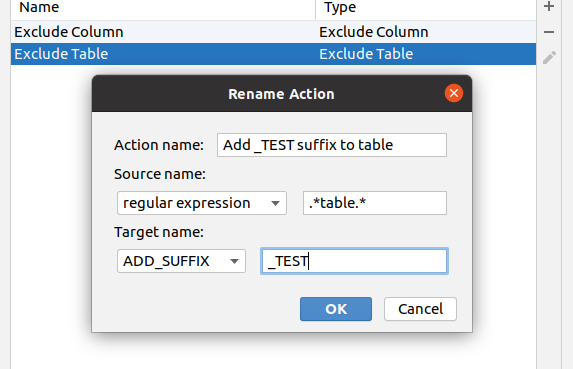
\includegraphics[width=0.5\textwidth]{images/ui/createRename}
		\caption{Migrationsoperation Umbenennen erstellen}
		\label{img:createRename}
	\end{figure}
	%Der reguläre Ausdruck \textbf{.*table.*} bedeutet im dargestellten Beispiel, dass die erstellte 

	Anschließend lässt sich die neu hinzugefügte Migrationsoperation durch einen Klick auf den ,Save‘-Button speichern (siehe Abbildung \ref{img:creategbaction})). Dabei werden alle Migrationsoperationen nach JSON konvertiert und in einer externen Datei gespeichert. Dafür ist die Klasse GsonHelper verantwortlich (siehe Abbildung \ref{img:gson}).
	\begin{figure}[h]
		\centering
		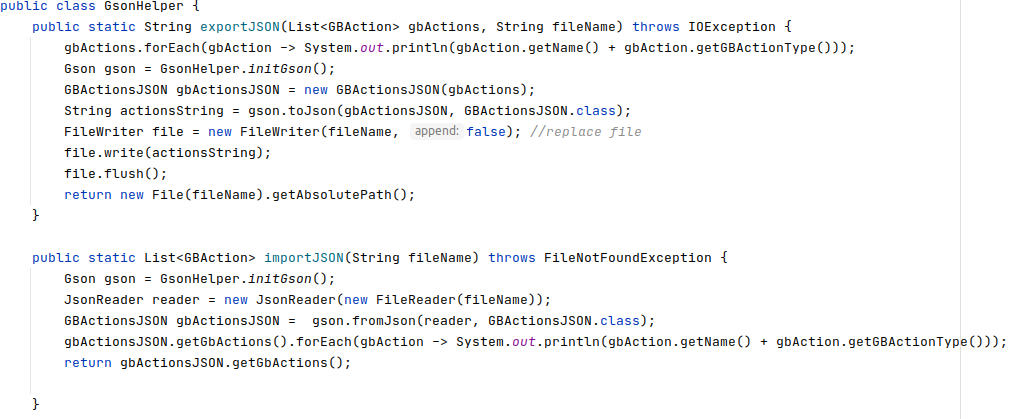
\includegraphics[width=0.9\textwidth]{images/ui/gson}
		\caption{Migrationsoperationen exportieren und importieren}
		\label{img:gson}
	\end{figure}
	
\subsection{Funktion: Verbindungerstellung}
		
	Wenn die Quell- und die Zieldatenbank im Database-Plugin eingerichtet sind, kann das Aktionsmenü nach einem Rechtsklick auf die Quelldatenbank aktiviert werden. Wie in  Abbildung \ref{img:dbactions} angezeigt wird, kann der Benutzer auf den Button ,Migrate Database‘ klicken, um die Übersicht der Datenbankmigration zu öffnen (siehe Abbildung \ref{img:ui:generalView}). Dabei wird die Quelldatenbank anhand der selektierten Datenbank automatisch ausgewählt. Außerdem müssen das zu migrierende Schema der Quelldatenbank sowie das Zielschema ausgewählt werden. Zusätzlich müssen die Zugangsdaten jeder Datenbank angegeben werden, um die Datenbanken zu verbinden. 
	

	\begin{figure}[h]
		\centering
		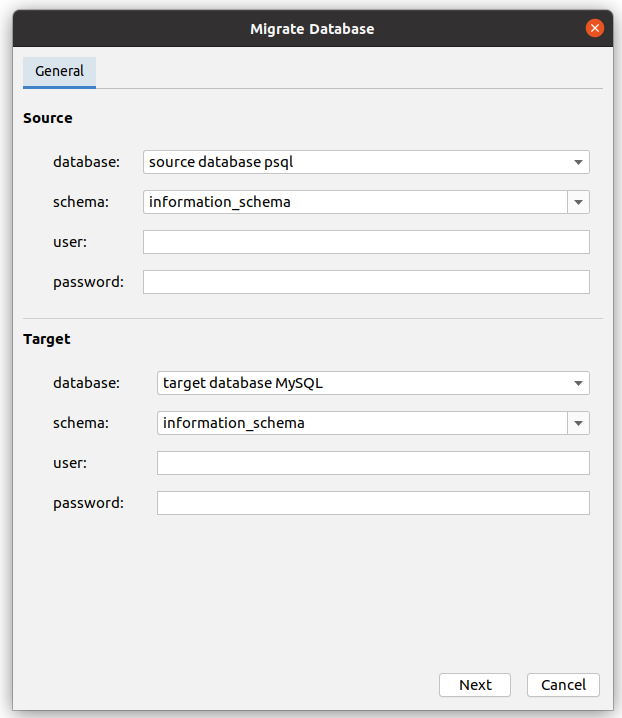
\includegraphics[width=0.5\textwidth]{images/ui/generalView}
		\caption{Allgemeine Übersicht über die Datenbankmigration (GeneralView)}
		\label{img:ui:generalView}
	\end{figure}
	
		Nach dem Klick auf den ,Next‘-Button werden die Angaben geprüft. Wenn sie fehlerhaft sind, wird eine entsprechende Fehlermeldung ausgegeben. Ansonsten wird das Connector-Repository (siehe \ref{sec:imp:gb}) anhand der angegebenen Informationen erstellt und anschließend wird die nächste Übersicht (Overview) angezeigt.
	
\subsection{Funktion: Konfiguration}	
	In der Konfigurationsübersicht (siehe Abbildung \ref{img:ui:overviewSingleAdd}) werden alle Elemente der Quelldatenbank angezeigt. Dabei sind eine Einzel- sowie eine Mehrfachauswahl möglich. \\
	\begin{figure}[h]
		\centering
		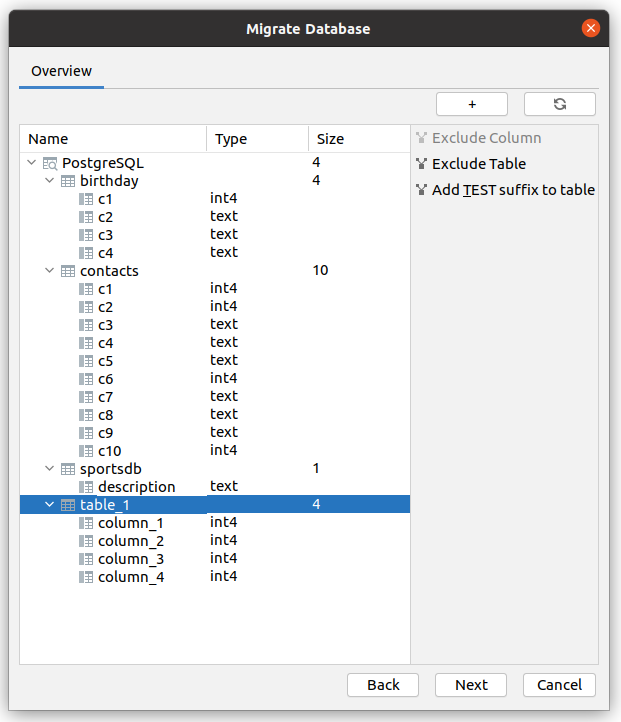
\includegraphics[width=0.5\textwidth]{images/ui/overviewSingleAdd}
		\caption{Konfigurationsübersicht (Overview)}
		\label{img:ui:overviewSingleAdd}
	\end{figure}
	Außerdem werden alle Migrationsoperationen mithilfe der Gson-Helper-Klasse geladen. Diese werden abhängig von den selektierten Elementen unterschiedlich dargestellt. Wenn eine Migrationsoperation (GBAction) zu den ausgewählten Elementen passt, wird sie klickbar angezeigt, ansonsten wird sie deaktiviert und ausgegraut dargestellt. Dabei spielt die Matches-Methode der GB-Action-Klasse eine entscheidende Rolle. Diese wird entsprechend dem Typ der Migrationsoperation implementiert. Für das Umbenennen wird z. B. geprüft, ob der gespeicherte reguläre Ausdruck zum Namen der selektierten Elemente passt (siehe Abbildung \ref{img:ui:matches}).
	
	\begin{figure}[h]
		\centering
		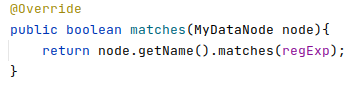
\includegraphics[width=0.5\textwidth]{images/ui/matches}
		\caption{Matches-Methode der Migrationsoperation Umbenennen}
		\label{img:ui:matches}
	\end{figure}
	Bei jedem Hinzufügen wird die entsprechende Migrationsoperation der Liste aller Operationen hinzugefügt. Dabei wird eine neue Instanz erzeugt, die die benötigten Informationen des entsprechenden Datenbankelementes enthält (\ref{img:ui:overviewAddRenameSrc}).
	%overviewAddRenameSrc
	\begin{figure}[H]
		\centering
		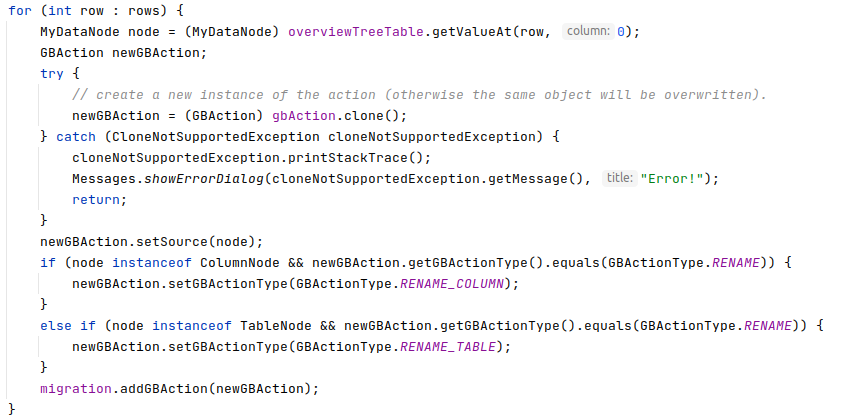
\includegraphics[width=0.9\textwidth]{images/ui/overviewAddRenameSrc}
		\caption{Hinzufügen der Migrationsoperation ,Umbenennen‘}
		\label{img:ui:overviewAddRenameSrc}
	\end{figure}
\subsection{Funktion: Migrationsdurchführung}
	
	Nach einem Klick auf den ,Next‘-Button erhält der Benutzer eine Übersicht über alle hinzugefügten Migrationsoperationen (siehe Abbildung \ref{img:ui:resultView}). Diese können nach Bedarf gelöscht werden. \\
	\begin{figure}[H]
		\centering
		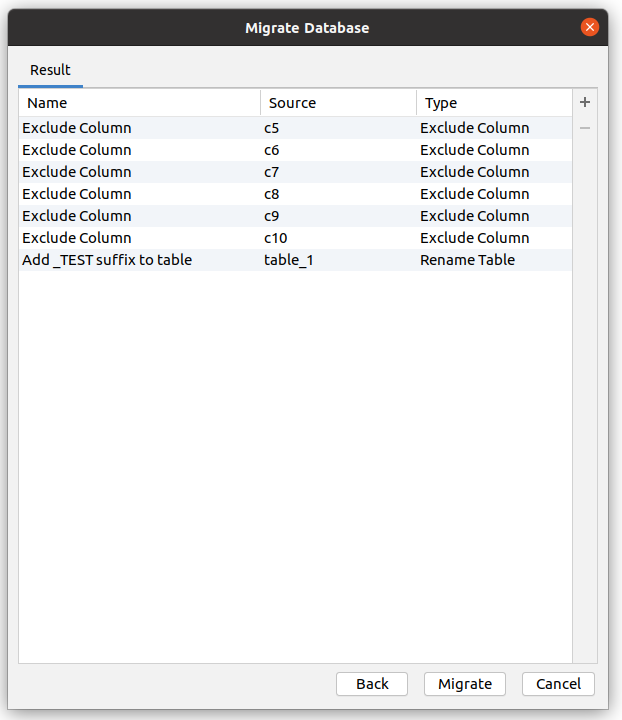
\includegraphics[width=0.5\textwidth]{images/ui/resultView}
		\caption{Ergebnisübersicht}
		\label{img:ui:resultView}
	\end{figure}
	Nach einem Klick auf den ,Migrate‘-Button wird die Fortschrittsübersicht angezeigt (siehe Abbildung \ref{img:ui:progressView}). Diese veranschaulicht den Migrationsprozess, der in einem neuen Thread ausgeführt wird. Bei der Migration werden die Mapper-Klassen sowie die GuttenBase-Connectors (siehe Abschnitt \ref{sec:imp:gb}) entsprechend den hinzugefügten Migrationsoperationen dem Connector-Repository hinzugefügt. Danach werden die Daten von der Quelldatenbank zur Zieldatenbank kopiert (siehe Abbildung \ref{img:ui:connectors} bzw. Abbildung \ref{img:ui:run}). \\
	\begin{figure}[H]
		\centering
		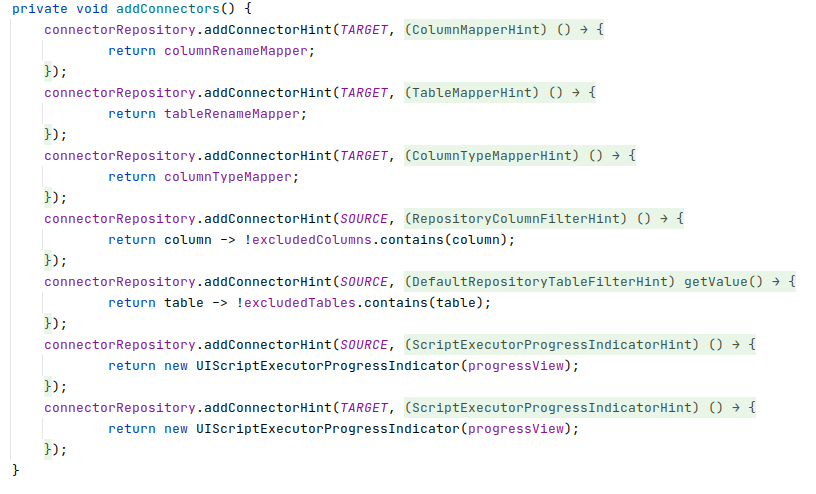
\includegraphics[width=0.9\textwidth]{images/ui/connectors}
		\caption{ConnectorHints hinzufügen}
		\label{img:ui:connectors}
	\end{figure}
	\begin{figure}[H]
		\centering
		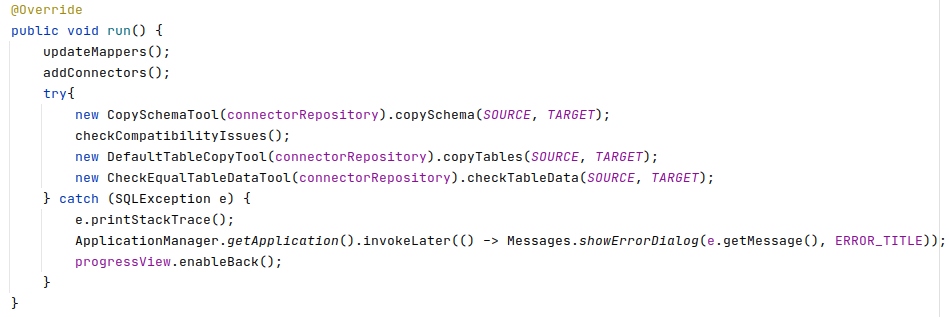
\includegraphics[width=0.9\textwidth]{images/ui/run}
		\caption{Migration durchführen (MapperHelper Klasse)}
		\label{img:ui:run}
	\end{figure}
	Falls ein Fehler bei der Migration auftritt, wird eine entsprechende Fehlermeldung angezeigt und das ‚Back‘ aktiviert, um Änderungen durchzuführen und die Migration abermals zu starten. Der Benutzer bekommt außerdem einen Hinweis, sobald die Migration erfolgreich abgeschlossen worden ist.
	
	\begin{figure}[H]
		\centering
		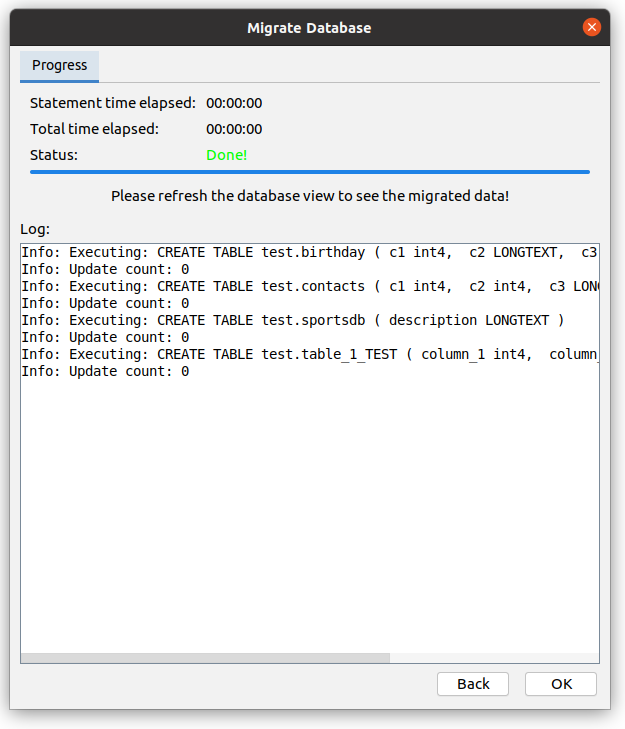
\includegraphics[width=0.5\textwidth]{images/ui/progressView}
		\caption{Fortschrittsübersicht}
		\label{img:ui:progressView}
	\end{figure}
%\subsection{Test}
%Für all der erläuterten Funtionen wurde manuelle Tests durchgeführt. Die Testdurchführung sowie die erwarteten Ergebnisse sind wie obenbeschrieben. Für die Testvorbereitung muss auf folgende Punkte geachtet werden:
%\begin{itemize}
%	\item Intellij starten.
%\end{itemize}